\documentclass[../../topologia_algebraica]{subfiles}
\begin{document}
\section{Complejos Simpliciales}

\subsection{Complejos simpliciales geom\'etricos}

\begin{defin}
  Un subconjunto $\{a_0,a_1,\ldots,a_n\}\subset\RR^n$ es \emph{afin-independiente} (AI) si
  el conjunto de diferencias $\{a_1-a_0,\ldots,a_n-a_0\}$ es linealmente independiente en $\RR^n$. 
\end{defin}

En palabras esto significa que un conjunto $\{a_0,\ldots,a_n\}$ es AI si el conjunto $\{a_1,\ldots,a_n\}$
bajo la traslaci\'on $a_0\mapsto 0$, es linealmente independiente. En particular, si
$\{a_1,\ldots,a_n\}$ es linealmente independiente en $\RR^n$, entonces $\{0,a_1,\ldots,a_n\}$ es AI.

Observa que en la definici\'on de AI, puedo tomar cualquier espacio ambiente $\RR^N$ con la
condici\'on $N\geq n$.

\import{\directory}{ejercicios/44} %%%%%%%%%%%%%%%%%%%%%%%%%%%%%%%%%%%%%%%%%%%%%%%%%%%% EJERCICIO 44

Este ejercicio dice que la condici\'on AI es casi equivalente a la independencia lineal, la \'unica
restricci\'on es que los coeficientes de la combinaci\'on lineal (igualada a cero) deben sumar 0.
Esta condici\'on adicional literlamente ``traslada'' la condici\'on de independencia lineal al punto
$a_0$.

\begin{defin}
  Un \emph{n-simplejo geom\'etrico} en $\RR^N$ (en particular $N\geq n$) es un subconjunto
  $\sigma_n\subset\RR^N$ de la forma:
  \[
    \sigma_n=
    \left\{\sum_{i=0}^n\la_ia_i \right|%
    \left. \{a_0,\ldots,a_n\}\;\text{es AI,}\;\;\la_i\geq 0,\;\; \sum_{i=0}^n\la_i=1\right\}
  \]
  y se denota como $\sigma_n=\gen{a_0,\ldots,a_n}$ (ve la figura \ref{fig:nsimplejos_geometricos}).
\end{defin}

\begin{figure}[ht] %%%%%%%%%%%%%%%%%%%%%%%%%%%%%%%%%%%%%%%%%%%%%%%%%%%%%%% FIGURA NSIMPLEJOS_GEOMETRICOS
  \centering
  \caption{Ejemplos de $n$-simplejos geom\'etricos de dimensi\'on 1,2 y 3}
  \label{fig:nsimplejos_geometricos}
  \begin{subfigure}{0.3\textwidth}
    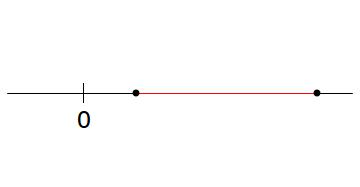
\includegraphics[scale=0.35]{1simplejo_geometrico}    
  \end{subfigure}
  \begin{subfigure}{0.3\textwidth}
    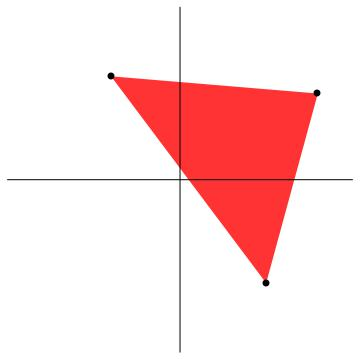
\includegraphics[scale=0.35]{2simplejo_geometrico}    
  \end{subfigure}
  \begin{subfigure}{0.3\textwidth}
    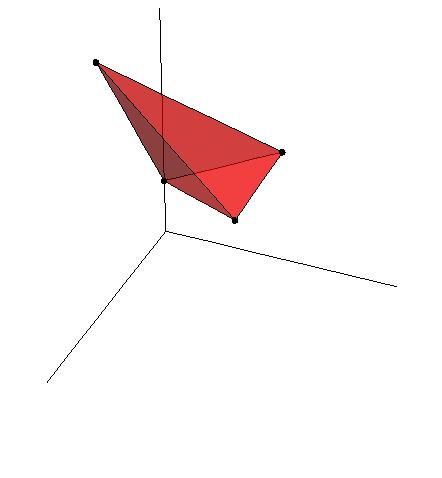
\includegraphics[scale=0.35]{3simplejo_geometrico}    
  \end{subfigure}
\end{figure}%%%%%%%%%%%%%%%%%%%%%%%%%%%%%%%%%%%%%%%%%%%%%%%%%%%%%%%%%%%%%%%%%%%%%%%%%%%%%%%%%%%%%%%%%%


\begin{nota}
  Esta definici\'on es exactamente la definici\'on de la cerradura convexa del conjunto
  $\{a_0,\ldots,a_n\}$, ie. $\text{Conv}(a_0,\ldots,a_n)=\gen{a_0,\ldots,a_n}$.
\end{nota}

Recuerda que la cerradura convexa de un conjunto $X\subset\RR^N$ (en este caso tomo
$X=\{x_1,\ldots,x_n\}$ finito) es la intersecci\'on de todos los conjuntos convexos que
lo contienen. M\'as precisamente si escribo
$\fC=\{Y\subseteq\RR^N\mid Y\;\text{es convexo y}\; X\subseteq Y\}$, entonces
\begin{equation}
  \label{eq:cerradura_convexa}
  \text{Conv}(X)=\bigcap_{Y\in\fC}Y.
\end{equation}

Es sencillo probar (\ref{eq:cerradura_convexa}): primero observa que $\text{Conv}(X)$ es un
conjunto convexo porque si $\la=\sum\la_ix_i,\mu=\sum\mu_ix_i\in\text{Conv}(X)$ entonces
\[
  t\la+(1-t)\mu=\sum_{i=1}^n(t\la_i+(1-t)\mu_i)x_i\in\text{Conv}(X) \quad\forall t\in[0,1]
\]
ya que
\[
  \sum_{i=1}^nt\la_i+(1-t)\mu_i=t\sum_{i=1}^n\la_i+(1-t)\sum_{i=1}^n\mu_i=t+(1-t)=1.
\]
Por lo tanto $\text{Conv}(X)\in\fC$ y la contenci\'on $\supseteq$ de (\ref{eq:cerradura_convexa})
se cumple.
Para la otra contenci\'on considera $Y\in\fC$ y observa que si $\sum\la_ix_i\in\text{Conv}(X)$
entonces $\sum\la_ix_i\in Y$ porque $x_1,\ldots,x_n\in Y$, $\sum\la_i=1$ y $Y$ es convexo; por lo
tanto $\text{Conv}(X)\subseteq Y$ para toda $Y\in\fC$.

Por \'ultimo, la intersecci\'on de conjuntos convexos es convexo (raz\'on: si $x,y\in\cap Y_i$ con
$Y_i$ convexo, entonces la recta $\Ll$ que un $x,y$ est\'a contenido en cada $Y_i$ y as\'i
$\Ll\subseteq \cap Y_i$), entonces he probado que:

\begin{prop}\label{prop:nsimplejo_geometrico_convexo}
  El $n$-simplejo geom\'etrico $\sigma=\gen{a_0,\ldots,a_n}$ es el conjunto convexo m\'as peque\~no
  que contiene al conjunto $\{a_0,\ldots,a_n\}$, en general:
  \[
    \sigma=\gen{a_0,\ldots,a_n}=\text{Conv}(a_0,\ldots,a_n)=\bigcap_{Y\in\fC}Y
  \]
  donde $\fC$ es la familia de conjuntos convexos $Y$ que contienen a $\{a_0,\ldots,a_n\}$.
\end{prop}

Hay una clase de $n$-simplejos muy importantes:

\begin{defin}
  El $n$-\emph{simplpejo geom\'etrico est\'andar}, denotado por $\Delta^n\subset\RR^{n+1}$, es el
  $n$-simplejo generado por la base can\'onica de $\RR^{n+1}$, ie. $\Delta^n:=\gen{e_0,\ldots,e_n}$.
\end{defin}

Ve la figura \ref{fig:nsimplejos_estandares} para los primeros ejemplos.

\begin{figure}[h!] %%%%%%%%%%%%%%%%%%%%%%%%%%%%%%%%%%%%%%%%%%%%%%%%%%%%%%% FIGURA NSIMPLEJOS_ESTANDAR
  \centering
  \caption{Ejemplos de $n$-simplejos geom\'etricos est\'andares de dimensi\'on 0,1 y 2}
  \label{fig:nsimplejos_estandares}
  \begin{subfigure}{0.3\textwidth}
    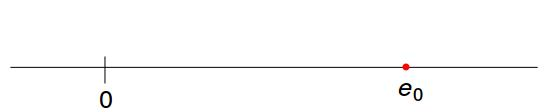
\includegraphics[scale=0.28]{0simplejo_estandar}    
  \end{subfigure}
  \begin{subfigure}{0.3\textwidth}
    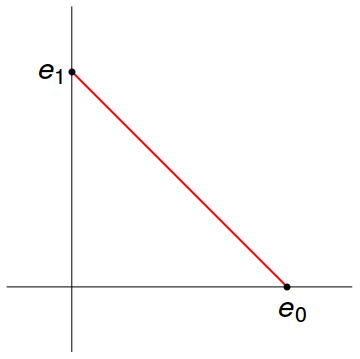
\includegraphics[scale=0.3]{1simplejo_estandar}    
  \end{subfigure}
  \begin{subfigure}{0.3\textwidth}
    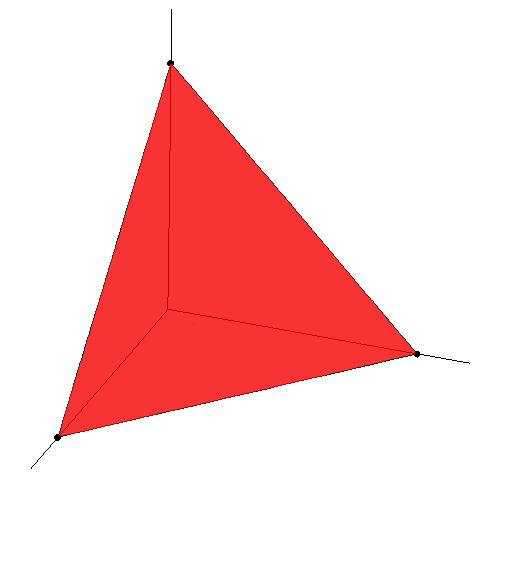
\includegraphics[scale=0.3]{2simplejo_estandar}    
  \end{subfigure}
\end{figure}%%%%%%%%%%%%%%%%%%%%%%%%%%%%%%%%%%%%%%%%%%%%%%%%%%%%%%%%%%%%%%%%%%%%%%%%%%%%%%%%%%%%%%%%%%

Observa que podemos encajar $\Delta^n$ en $\RR^n$ en lugar de $\RR^{n+1}$ como
$\Delta^n=\gen{0,e_1,\ldots,e_n}$; en este caso
$\Delta^n=\{(\la_1,\ldots,\la_n)\in\RR^n\mid \sum\la_i\leq 1,\;\la_i\geq 0\}$. Estas dos maneras de
definir los simplejos est\'andares son equivalentes entonces usar\'e ambas descripciones
intercambiablemente.

Los $n$-simplejos geom\'etricos est\'andares nos permite clasificar topol\'ogicamente todos los
$n$-simplejos geom\'etricos mediante la siguiente proposici\'on:

\begin{prop}\label{prop:clasificacion_simplejos_geometricos}
  Sean $\sigma=\gen{a_0,\ldots,a_n}$ y $\tau=\gen{b_0,\ldots,b_n}$ dos $n$-simplejos en $\RR^N$.
  Entonces $\sigma\approx\tau$ donde el homeomorfismo s\'olo depende de los v\'ertices. En este
  caso se dice que $\sigma$ y $\tau$ son \emph{afinmente homeomorfos}.
\end{prop}

\import{\directory}{ejercicios/46} %%%%%%%%%%%%%%%%%%%%%%%%%%%%%%%%%%%%%%%%%%%%%%%%% EJERCICIO 46

Un corolario inmediato de este ejercicio es que todo $n$-simplejo geom\'etrico
$\sigma=\gen{a_0,\ldots,a_n}$ es homeomorfo al complejo geom\'etrico est\'andar $\Delta^n$. Por lo
tanto la topolog\'ia de $\Delta^n$ completamente determina la topolog\'ia de los $n$-simplejos
geom\'etricos:

\import{\directory}{ejercicios/45} %%%%%%%%%%%%%%%%%%%%%%%%%%%%%%%%%%%%%%%%%%%%%%%%%% EJERCICIO 45

\begin{defin}
  Sea $\sigma=\gen{a_0,\ldots,a_n}$ un $n$-simplejo geom\'etrico y $m\leq n$. Una $m$-\emph{cara} $\tau$
  de $\sigma$ es el $m$-simplejo geom\'etrico asociado a alg\'un subconjunto $\{a_{i_0},\ldots,a_{i_m}\}$
  de $\{a_0,\ldots,a_n\}$, es decir $\tau=\gen{a_{i_0},\ldots,a_{i_n}}\subseteq\sigma$.
\end{defin}

\begin{defin}
  El \emph{baricentro} de un $n$-simplejo geom\'etrico $\sigma=\gen{a_0,\ldots,a_n}$ es el punto
  \[
    \fb(\sigma)=\frac{1}{n+1}\sum_{i=0}^{n}a_i
  \]
\end{defin}
Observa que el baricentro $\fb(\sigma)$ es un elemento de $\sigma$ porque $\sum\tfrac{1}{n+1}=1$.

Los $n$-simplejos por s\'i solos no son muy interesantes topolo\'ogicamente (acabamos de clasificarlos
todos!), pero forman parte de una construcci\'on muy importante:

\begin{defin}
  Un \emph{complejo simplicial geom\'etrico} en $\RR^N$ es una familia finita $K$ de simplejos
  geom\'etricos (de dimensi\'on $\leq N$) que cumple dos propiedades:
  \begin{enumerate}
  \item[($i$)] $K$ contiene todas las caras de todos sus elementos, es decir si $\sigma\in K$
    y $\tau\subset\sigma$ es una cara, entonces $\tau\in K$.
  \item[($ii$)] La intersecci\'on de cualesquiera dos $\sigma,\tau\in K$ es una cara com\'un de
    $\sigma$ y $\tau$ (tambi\'en incluyo el caso cuando la intersecci\'on es vac\'ia).
  \end{enumerate}
\end{defin}

Intuitivamente, la primera propiedad nada m\'as garantiza que est\'as trabajando con todos los
posibles sub-simplejos del complejo. La segunda condici\'on te dice que los simplejos se pegan
bien, es decir a lo largo de caras (que por la primera propiedad son elementos de $K$).

Para visualizar un complejo simplicial geom\'etrico $K$, dibjuamos su ``realizaci\'on geom\'etrica''
$\abs{K}:=\{x\in\RR^N\mid \exists\sigma\in K\;\text{tal que}\;x\in\sigma\}=\bigcup_{\sigma\in K}\sigma$.

\begin{figure}[ht] %%%%%%%%%%%%%%%%%%%%%%%%%%%%%%%%%%%%%%%%%%%%%%%%%%%%%%% FIGURA NSIMPLEJOS_GEOMETRICOS
  \centering
%  \caption{Ejemplos de $n$-simplejos geom\'etricos de dimensi\'on 1,2 y 3}
%  \label{fig:complejo_simplicial_geometrico}
  \begin{subfigure}{0.48\textwidth}\caption{S\'i es complejo simplicial geom\'etrico.}
    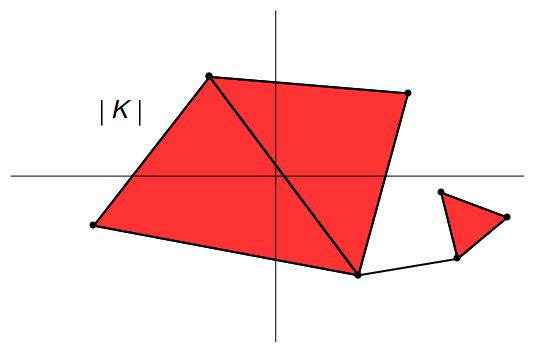
\includegraphics[scale=0.4]{complejo_simplicial_geometrico_si}    
  \end{subfigure}
  \begin{subfigure}{0.48\textwidth}\caption{No es complejo simplicial geom\'etrico.}
    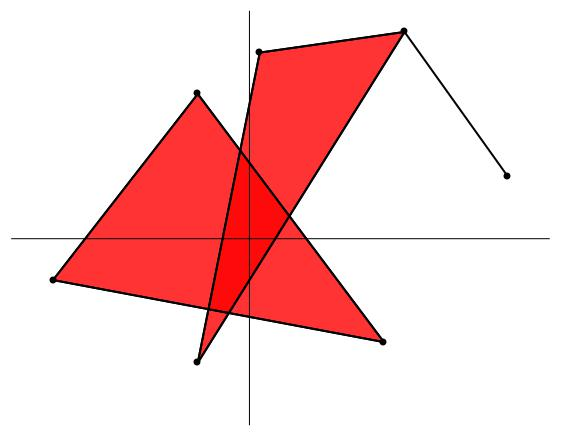
\includegraphics[scale=0.35]{complejo_simplicial_geometrico_no}    
  \end{subfigure}
\end{figure}%%%%%%%%%%%%%%%%%%%%%%%%%%%%%%%%%%%%%%%%%%%%%%%%%%%%%%%%%%%%%%%%%%%%%%%%%%%%%%%%%%%%%%%%%%

Esta construcci\'on se puede generalizar considerablemente.

\subsection{Complejos simpliciales abstractos}

\begin{defin}
  Une \emph{complejo simplicial} (abstracto) $K$ es una familia de subconjuntos finitos no vac\'ios
  de un conjunto $V_K$, cuyos elementos se llaman \emph{v\'ertices}, que satisface:
  \begin{enumerate}
    \item[($i$)] $K$ contiene todos los singuletes de $V_K$, es decir $v\in V_k\;\then\; \{v\}\in K$.
    \item[($ii$)] $K$ es cerrado bajo subconjuntos, es decir si $L\in K$ y $L'\subseteq L$ entonces
      $L'\in K$.
  \end{enumerate}
\end{defin}

Esta definici\'on efectivamente generaliza la definici\'on de complejo simplicial geom\'etrico; la
idea es que para pasar de complejos simpliciales geom\'etricos a complejos simpliciales abstractos
basta tomar los ``v\'ertices'' de los simplejos geom\'etricos en lugar de todas las combinaciones
convexas de ellas.

\import{\directory}{ejercicios/47} %%%%%%%%%%%%%%%%%%%%%%%%%%%%%%%%%%%%%%%%%%%%%%%%%% EJERCICIO 47

Cada complejo simplicial $K$ tiene una realizaci\'on topol\'ogica, ie. tiene asociado can\'onicamente
un espacio topol\'ogico que se denota por $\abs{K}$.

\begin{defin}
  Sea $K$ un complejo simplicial con conjunto de v\'ertices $V_K$, entonces se define:
  \[
    \abs{K}:=
    \left\{\sigma:V_K\ra I\subset\RR : \sigma^{-1}(0,1]\in K,\;\;\sum_{v\in V_K}\sigma(v)=1\right\}\subset
    \{f:V_K\ra\RR\}=\RR^{V_K}
  \]
  que tiene una m\'etrica definida por:
  \[
    d:\abs{K}\times\abs{K} \ra \RR \quad,\quad d(\sigma,\tau)=\sqrt{\sum_{v\in V_K}(\sigma(v)-\tau(v))^2}.
  \]
  El espacio topol\'ogico inducido por esta m\'etric se denota por $\abs{K}_d$.
\end{defin}

Observa que las sumas en la definici\'on anterior est\'an bien definidas porque para $\sigma\in\abs{K}$
se tiene que $\sigma(v)\neq 0$ para s\'olo una cantidad finita de v\'ertices ya que por definici\'on
$\{v\in V_K\mid \sigma(v)\neq 0\}=\sigma^{-1}(0,1]\in K$ y los elementos de $K$ son conjuntos finitos.

\begin{nota}
  El conjunto $\sigma^{-1}(0,1]$ es exactamente el soporte de la funci\'on $\sigma$, ie.
  \[
    \sigma^{-1}(0,1]=\text{Sop}(\sigma):=\{v\in V_K\mid \sigma(v)\neq 0\}.
  \]
  Entonces usar\'e ambas descripciones intercambiablemente.
\end{nota}

\import{\directory}{ejercicios/48} %%%%%%%%%%%%%%%%%%%%%%%%%%%%%%%%%%%%%%%%%%%%%%% EJERCICIO 48

Aunque la definici\'on de $\abs{K}$ parece complicada, s\'i concuerda con la intuici\'on,
especialmente cuando $V_K$ es finito. Por ejemplo:

\begin{ejemplo}\label{ejemplo:complejo_circulo}
  Sea $V_K=\{0,e_1,e_2\}\subset\RR^2$ y $K=\{\{0\},\{e_1\},\{e_2\},\{0,e_1\},\{0,e_2\},\{e_1,e_2\}\}$.
  Como $V_K$ es finito (con tres elementos), entonces una funci\'on $\sigma:V_K\ra I$ la puedo
  representar como una terna $\sigma=(\sigma(0),\sigma(e_1),\sigma(e_2))$. Como $V_K\not\in K$ entonces
  al menos una coordenada de $\sigma$ debe ser 0. Por lo tanto, la segunda propiedad que cumple
  $\sigma$, (ie. la suma de las tres coordenadas da 1) me permite describir completamente $\abs{K}$.
  Por ejemplo si $\sigma(0)=0$ entonces $\sigma(e_1)=1-\sigma(e_2)$, por lo tanto cualquier
  $\sigma\in\abs{K}$ que cumple que $\sigma(0)=0$ est\'a completamente determinado por un par\'ametro
  $t=\sigma(e_1)\in I$, es decir $\sigma=(0,t,1-t)$. De esta manera tengo que:
  \[
    \abs{K}=
    \{(0,t,1-t)\mid t\in\RR \}\bigcup
    \{(t,0,1-t)\mid t\in\RR \}\bigcup
    \{(t,1-t,0)\mid t\in\RR \}
  \]
  que es la orilla de $\Delta^2\subset\RR^3$. %
  %
  \begin{figure}[h!]%%%%%%%%%%%%%%%%%%%%%%%%%%%%%%%%%%%%%%%%%%%%%%%%%%%%%%%% FIGURA COMPLEJO_CIRCULO
    \centering
    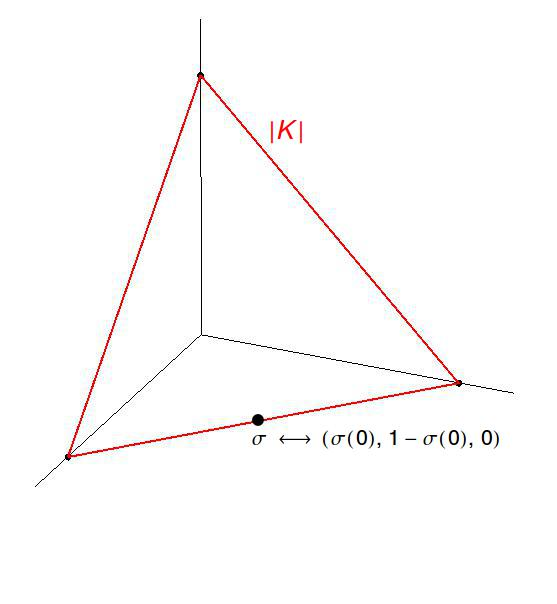
\includegraphics[trim=40 100 40 50, clip,scale=0.4]{complejo_circulo}
  \end{figure}%%%%%%%%%%%%%%%%%%%%%%%%%%%%%%%%%%%%%%%%%%%%%%%%%%%%%%%%%%%%%%%%%%%%%%%%%%%%%%%%%%%%%%
  %
  Tambi\'en observa que la m\'etrica $d$ de $\abs{K}$ coincide con la m\'etrica usual de $\RR^3$
  ya que los sumandos $\sigma(v)-\tau(v)$ dentro del radical son simplemente las diferencias
  de las coordenadas de $\sigma$ y $\tau$ vistas como puntos en $\RR^3$.
\end{ejemplo}

Como el caso finito es sencillo, formalizo este caso:

\begin{defin}
  Sea $K$ un complejo simplicial y $L\in K$, entonces
  \[
    \abs{L}:=
    \{\sigma\in\abs{K}:\sigma^{-1}(0,1]\subseteq L\}=
    \{\sigma\in \abs{K}:\text{Sop}(\sigma)\subseteq L\}.
  \]
\end{defin}

La importancia de analizar $\abs{L}$ para $L\in K$ es evidente del siguiente ejercicio:

\import{\directory}{ejercicios/49} %%%%%%%%%%%%%%%%%%%%%%%%%%%%%%%%%%%%%%%%%%%%%%% EJERCICIO 49

\begin{nota}
  Observa que $\abs{K}$ es la uni\'on de todos los subespacios $\abs{L}$, entonces el ejercicio
  anterior prueba que:
  \[
    \abs{K}=\bigcup_{L\in K}\abs{L}\approx \bigcup \Delta^n,
  \]
  es decir que la realizaci\'on topol\'ogica de un complejo simplicial es una uni\'on de simplejos
  geom\'etricos est\'andares.
\end{nota}

El ejercicio \ref{ej:49} y la nota anterior nos permite definirle una topolog\'ia a $\abs{K}$ sin
mencionar m\'etricas:

\begin{defin}
  Sea $K$ un complejo simplicial. Para cada $L\in K$, as\'ignale a $\abs{L}$ la topolog\'ia
  inducida por el homeomorfismo $\abs{L}\approx\Delta^n$. Entonces la \emph{topolog\'ia coherente}
  de $\abs{K}$ est\'a definido por:
  \[
    U\subseteq\abs{K}\;\;\text{es abierto} \quad\iff\quad
    U\cap\abs{L}\;\;\text{es abierto}\;\;\forall L\in K
  \]
\end{defin}

\begin{nota}
  De ahora en adelante, $\abs{K}$ se refiere a la realizaci\'on topol\'ogica del complejo simplicial
  $K$ con la topolog\'ia coherente y $\abs{K}_d$ a la realizaci\'on topol\'ogica con la topolog\'ia
  inducida por la m\'etrica $d$ del ejercicio \ref{ej:48}.
\end{nota}

\begin{nota}
  Vale la pena mencionar que una funci\'on $f:\abs{K}\ra X$ es continua si y s\'olo si
  $f|_{\abs{L}}:\abs{L}\ra X$ es continua para toda $L\in K$. Esto quiere decir que
  $\Id:\abs{K}\ra\abs{K}_d$ es continua porque $\Id|_{\abs{L}}:\abs{L}\ra\abs{L}_d$ es continua por
  definici\'on de la topolog\'ia de $\abs{L}$ (como $\abs{L}\approx\Delta^n\subset\RR^{n+1}$, la
  m\'etrica $d$ restringida a $\abs{L}$ coincide exactamente con la euclideana de $\RR^{n+1}$).
  Por lo tanto la topolog\'ia coherente es m\'as fina que la topol\'ogia inducida por la m\'etrica
  $d$, es decir tiene m\'as abiertos.
\end{nota}

\begin{defin}
  Un complejo simplicial $K$ es \emph{localmente finito} si para cada $v\in V_K$ s\'olo hay una
  cantidad finita de $L\in K$ tales que $v\in L$, es decir que el conjunto $\{L\in K\mid v\in L\}$
  es finito para todo v\'ertice $v$.
\end{defin}
 
La importancia de esta condici\'on se muestra en el siguiente teorema:

\begin{thm}
  Sea $K$ un complejo simplicial. Las siguientes proposiciones son equivalentes:
  \begin{enumerate}
  \item $K$ es localmente finito.
  \item $\abs{K}$ es compacto.
  \item $\Id:\abs{K}\ra\abs{K}_d$ es un homeomorfismo, es decir que la topolog\'ia coherente
    coincide con la toplog\'ia inducida por la m\'etrica $d$.
  \item $\abs{K}$ es metrizable.
  \item $\abs{K}$ satisface el primer axioma de numerabilidad, ie. todo punto $\sigma\in\abs{K}$
    tiene una base local numerable.
  \end{enumerate}
\end{thm}

\subsection{Triangulaciones y nervios}

\begin{defin}
  Un espacio $X$ es \emph{triangulable} si existe un complejo simplicial $K$ tal que
  $\abs{K}\approx X$.
\end{defin}

\import{\directory}{ejercicios/50} %%%%%%%%%%%%%%%%%%%%%%%%%%%%%%%%%%%%%%%%%%%%%%%%%%%%%% EJERCICIO 50

Este ejercicio se generaliza a variedades:

\begin{thm}
  Toda variedad suave es triangulable.
\end{thm}

Ahora doy un ejemplo de un complejo simplicial abstracto:

\begin{defin}(Alexandrov y $\check{\text{C}}$ech)
  Sean $X$ un espacio topol\'ogico y $\Cc=\{C_j\}_{j\in J}$ una familia de subespacios (en general
  se toma una cubierta abierta). El \emph{nervio} de $\Cc$, denotado por $\Nn\Cc$ es el complejo
  simplicial con v\'ertices $V_{\Nn\Cc}=J$, el conjunto de \'indices, y $n$-simplejos de la forma
  $L=\{j_0,\ldots,j_n\}$ donde $C_{j_0}\cap\cdots\cap C_{j_n}\neq\emptyset$.
\end{defin}

Por ejemplo, un sub-complejo simplicial de un nervio se puede ver como:

\begin{figure}[h!]%%%%%%%%%%%%%%%%%%%%%%%%%%%%%%%%%%%%%%%%%%%%%%%%%%%%%%%%%%%%%%%%%%%%%%% FIGURE
  \centering
  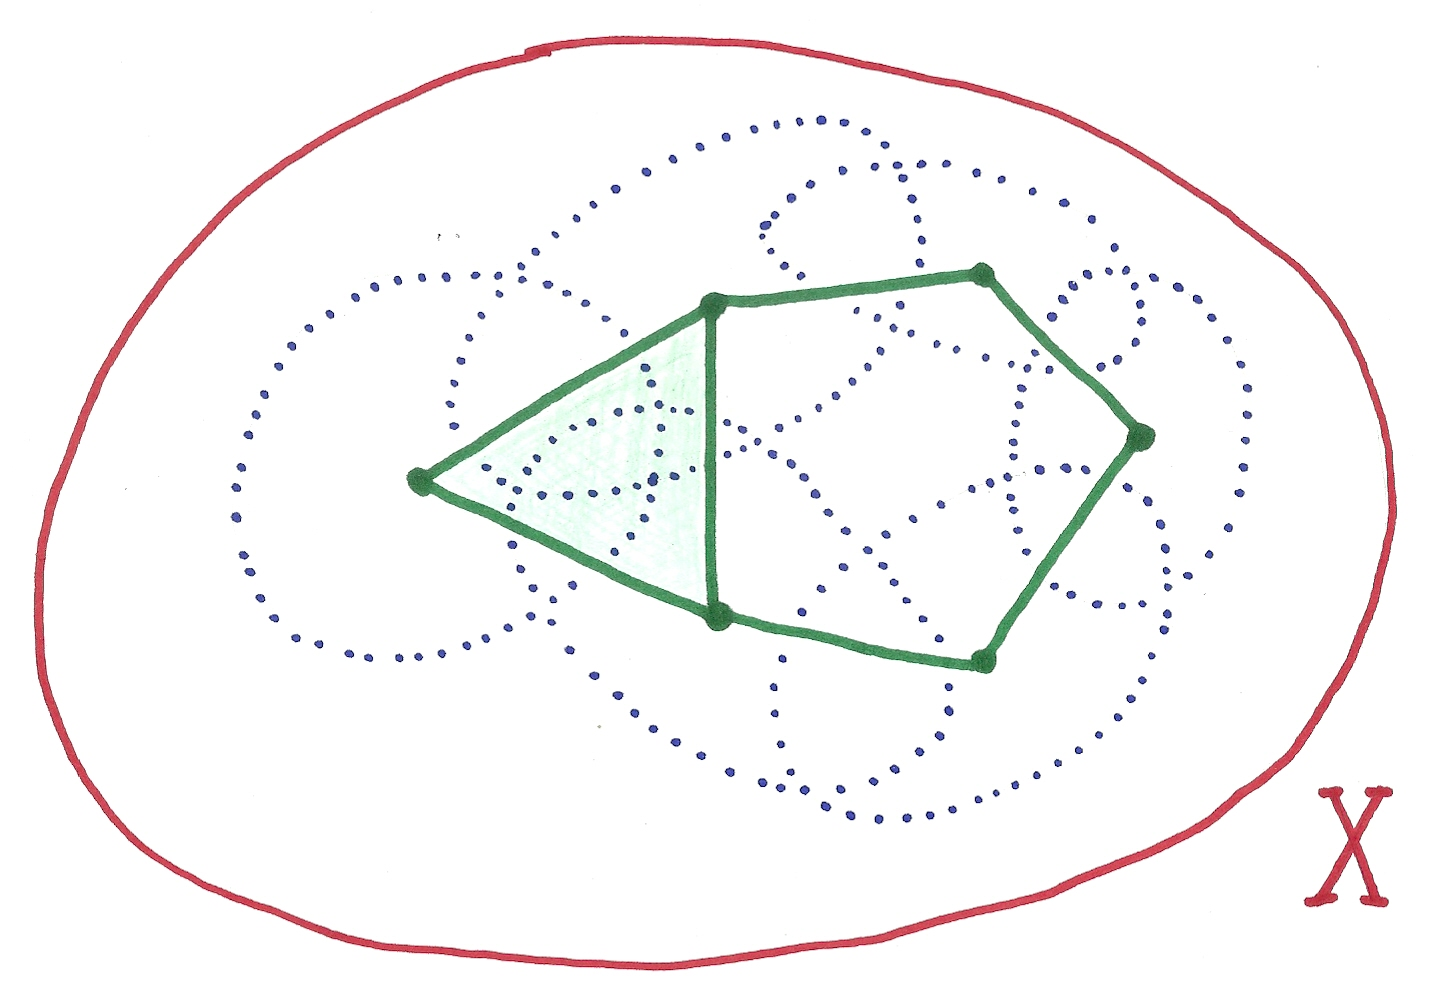
\includegraphics[scale=0.11]{complejo_nervio}
\end{figure}%%%%%%%%%%%%%%%%%%%%%%%%%%%%%%%%%%%%%%%%%%%%%%%%%%%%%%%%%%%%%%%%%%%%%%%%%%%%%%%%%%%%






\subsection{Homolog\'ia Simplicial}

Primero estudio la orientaci\'on de los complejos simpliciales.

\begin{defin}
  Sea $K$ un complejo simplicial y $\sigma\in K$ un $n$-simplejo. Adem\'as sea $\Sigma=\Sigma(\sigma)$
  el conjunto de funciones biyectivas $\underline{n}\lra\sigma$, donde
  $\underline{n}=\{0,\ldots,n\}\subset\NN$. Entonces hay una relaci\'on de equivalencia:
  \[
    f \simeq g \quad\iff\quad g^{-1}f\in S_{n+1}\;\;\text{es una permutaci\'on par.}
  \]
\end{defin}

\import{\directory}{ejercicios/51} %%%%%%%%%%%%%%%%%%%%%%%%%%%%%%%%%%%%%%%%%%%%%%% EJERCICIO 51

En la prueba del ejercicio anterior se vi\'o que $\Sigma(\sigma)/_{\sim}$ tiene naturalmente
una estructura de grupo isomorfa a $\ZZ_{2}$ bajo el isomorfismo (continuo) $[f]\mapsto1$ y
$[\bar{f}]\mapsto-1$. Entonces, $\Sigma(\sigma)/_{\sim}\cong\{1,-1\}$.

\begin{defin}
  Sea $K$ un complejo simplicial y $\sigma\in K$ un $n$-simplejo. Una \emph{orientaci\'on} de
  $\sigma$ es la pareja $(\sigma,\fo_{\sigma})$ donde $\fo_{\sigma}\in\Sigma(\sigma)/_{\sim}=\{1,-1\}$.
\end{defin}

En variedades triangulables, las orientaciones de los complejos simpliciales que realizan a la variedad
cumplen varias propiedades importantes.

Sea $M^n$ una variedad compacta de dimensi\'on $n$ con triangulaci\'on $M\approx\abs{K}$. Entonces
cada simplejo de $K$ es cara de un $n$-simplejo y adem\'as cada $(n-1)$-simplejo es cara de
exactamente dos $n$-simplejos. Estas dos propiedades permiten definir orientaci\'on de complejos
simpliciales que realizan variedades compactas.

\begin{defin}
  Sea $M^n$ una variedad suave y compacta tal que $M\approx\abs{K}$ para alg\'un complejo
  simplicial $K$. Una \emph{orientaci\'on} de $K$ es una elecci\'on de una orientaci\'on
  para cada $n$-simplejo $\sigma\in K$, que cumple que las dos orientaciones inducidas en cada
  $(n-1)$-simplejo de $K$ son distintas.
\end{defin}

M\'as precisamente, cada $(n-1)$-simplejo $\sigma\in K$ es cara de exactamente dos $n$-simplejos
$\tau,\tau'\in K$. Entonces la orientaciones $\fo_{\tau}$ y $\fo_{\tau'}$ deben ser distintas, ie.
$\fo_{\tau}=-\fo_{\tau'}$.

\begin{figure}[h!]%%%%%%%%%%%%%%%%%%%%%%%%%%%%%%%%%%%%%%%%%%%%%%%%%%%%%%%%%%%%%%%%%%%%%%% FIGURE
  \centering
%  \includegraphics[scale=0.11]{orientacion_triangulacion}
\end{figure}%%%%%%%%%%%%%%%%%%%%%%%%%%%%%%%%%%%%%%%%%%%%%%%%%%%%%%%%%%%%%%%%%%%%%%%%%%%%%%%%%%%%

\begin{ejemplo}
  Toma $\SS^1$ que es triangulable mediante el complejo simplicial $K$ (cf. ejercicio \ref{ej:50}).
  Entonces los 1-simplejos son $\{e_0,e_1\},\{e_1,e_2\},{e_2,e_0}$ (el orden dado los dota de una
  orientaci\'on a cada una).
\end{ejemplo}
\end{document}